\subsection{VoIP}

To configure the \gls{voip} service on the \gls{crg}s, a similar process to the manual Internet setup is followed on both equipment. There is no difference in this process on copper-based and fiber-based devices.

The \gls{sip} configuration collected from all \glspl{cpe} show that an outbound proxy is always used. This proxy is located at \url{192.168.80.1} and is only accessible on a network with \gls{vlan} \gls{id} different from the one used for the Internet Connection.

\begin{figure}[h]
    \centering
    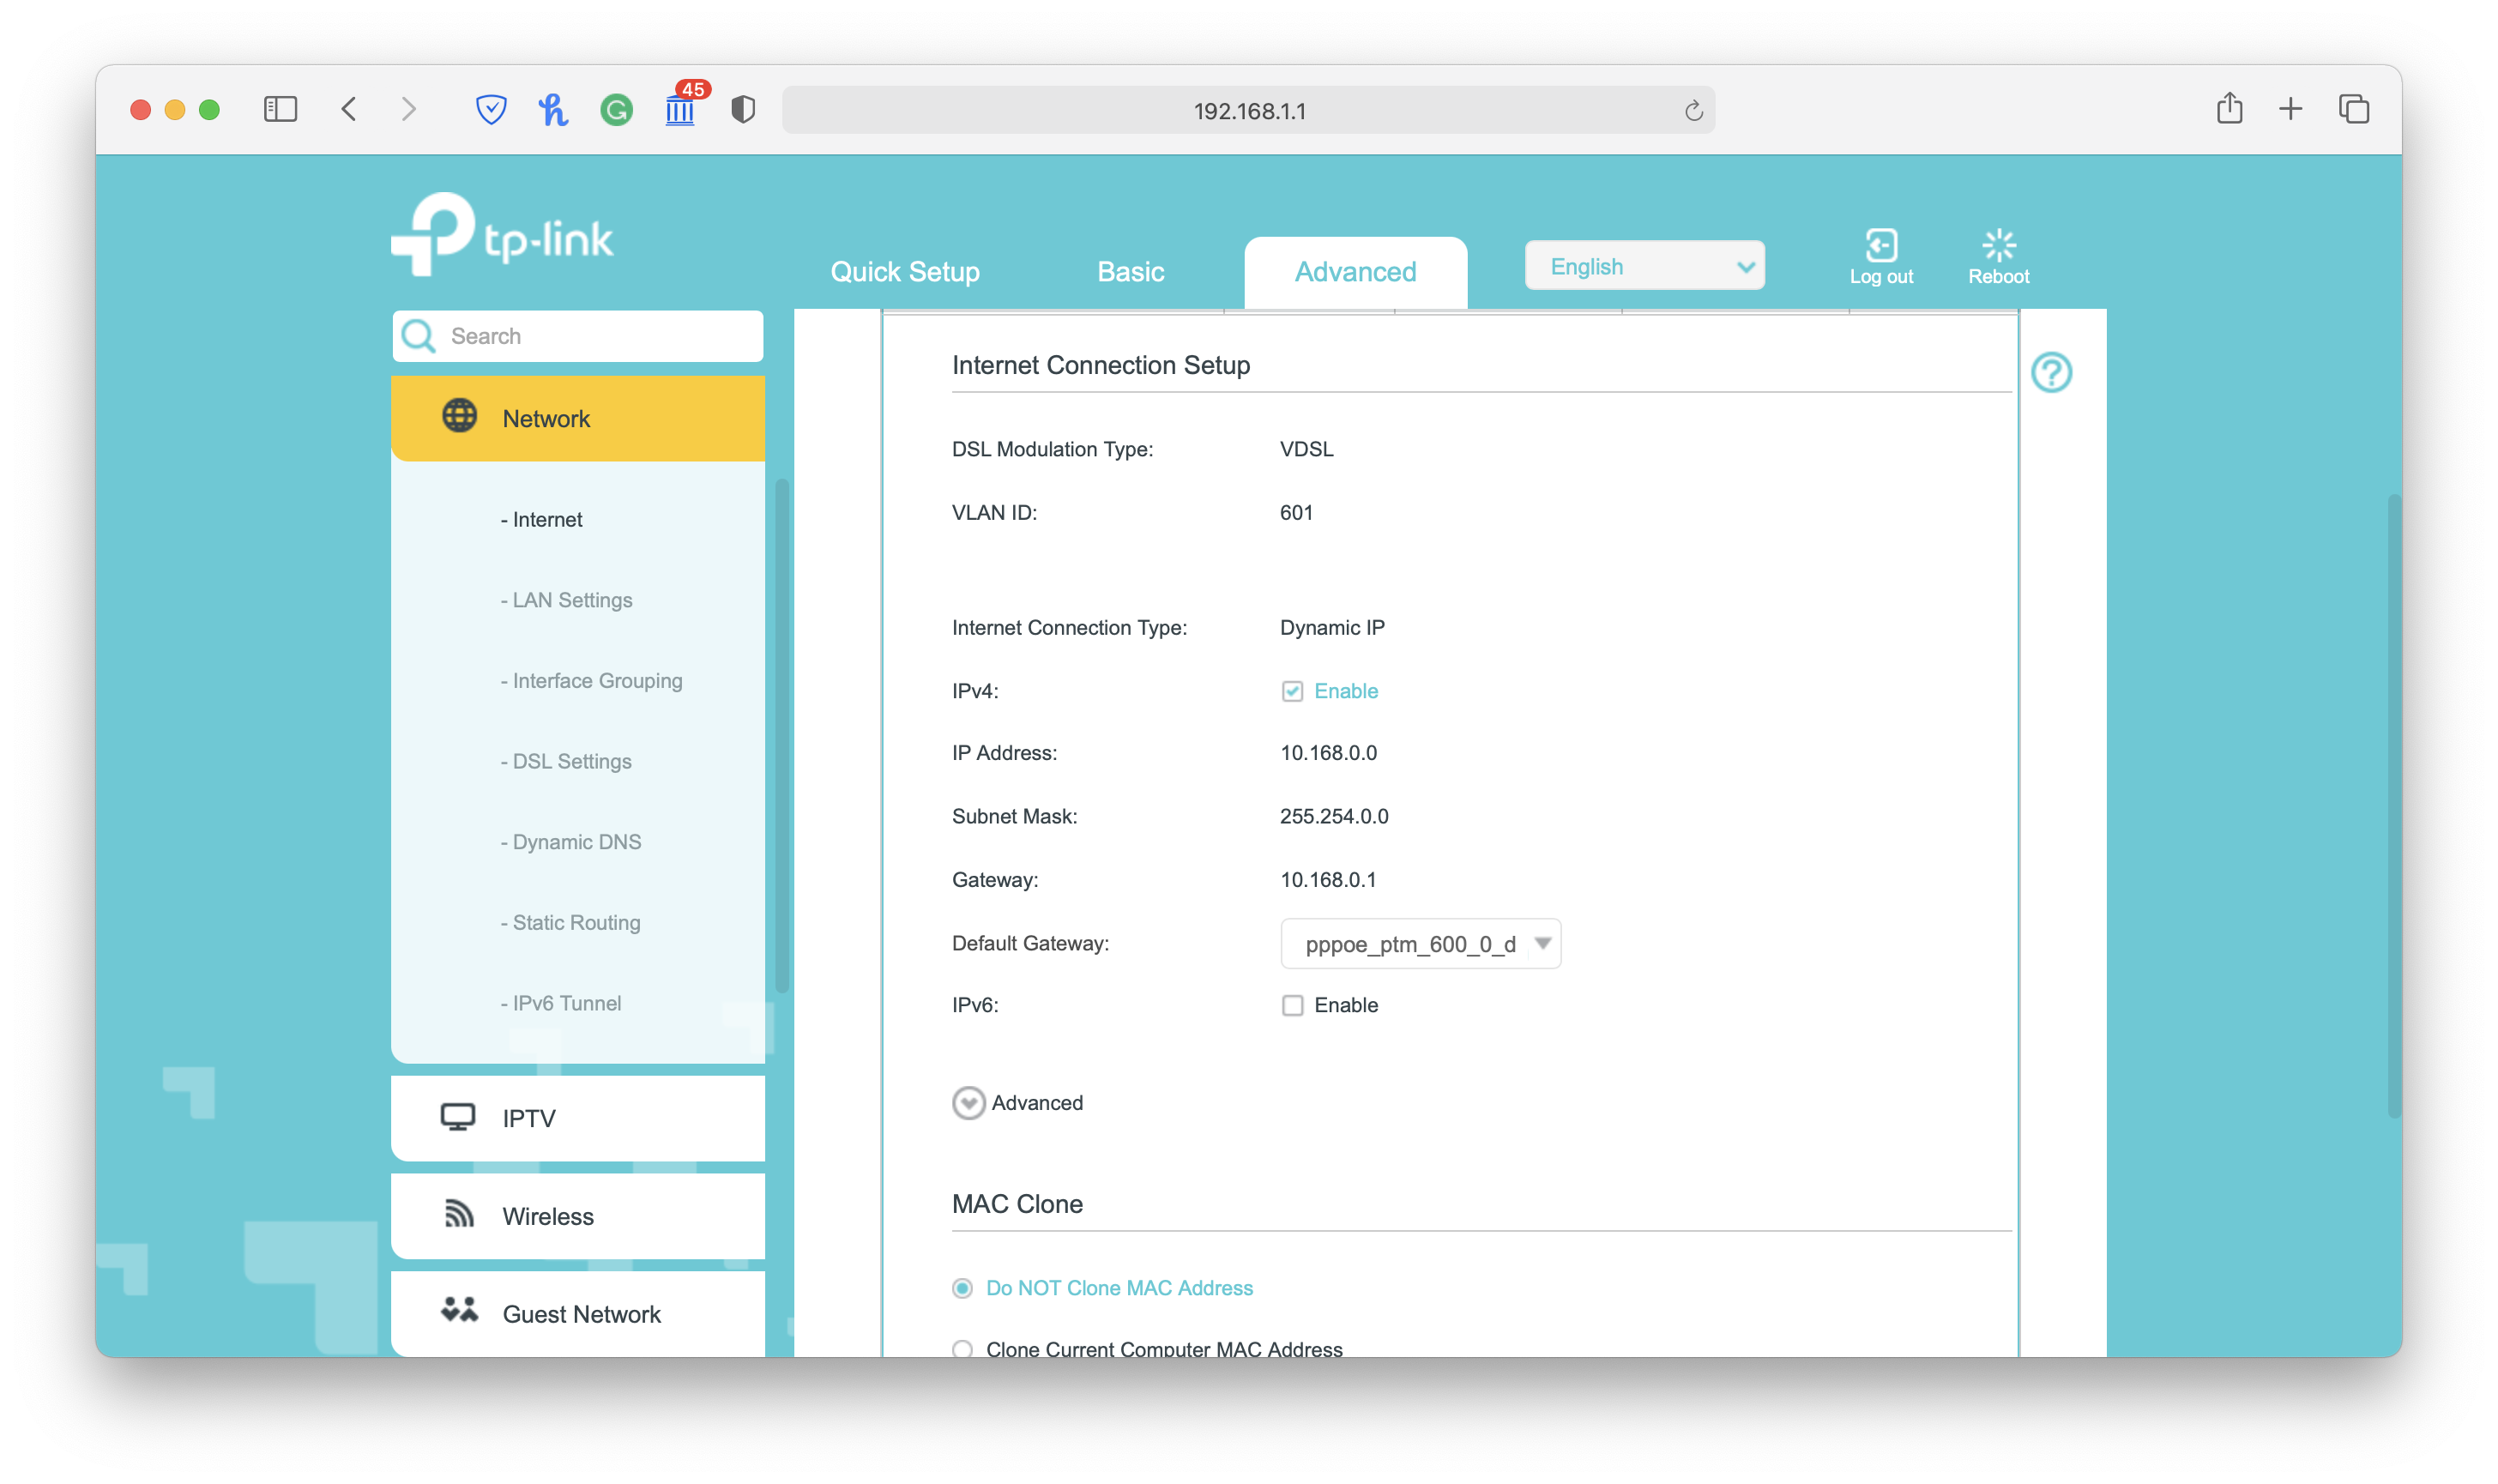
\includegraphics[width=\linewidth]{contents/substituting-the-isp-cpe/voip/advanced-network-internet-vlan601.png}
    \caption{\gls{vlan} 601 Settings of the \gls{crg}s}
    \label{figure:crgs_vlan601}
\end{figure}

Then, the Internet Configuration page must be accessed and a new connection created. The \gls{vlan} \gls{id} must be set to 601 and the Connection Type to Dynamic \gls{ip}, as shown in Figure \ref{figure:crgs_vlan601}. The default gateway must not be changed and \gls{ip}v6 must not be enabled.

After creating this new connection, an \gls{ip} address is automatically acquired. The joined network is part of the \url{10.0.0.0/8} \gls{ip}v4 range and doesn’t provide access to the Internet.

\begin{figure}[h]
    \centering
    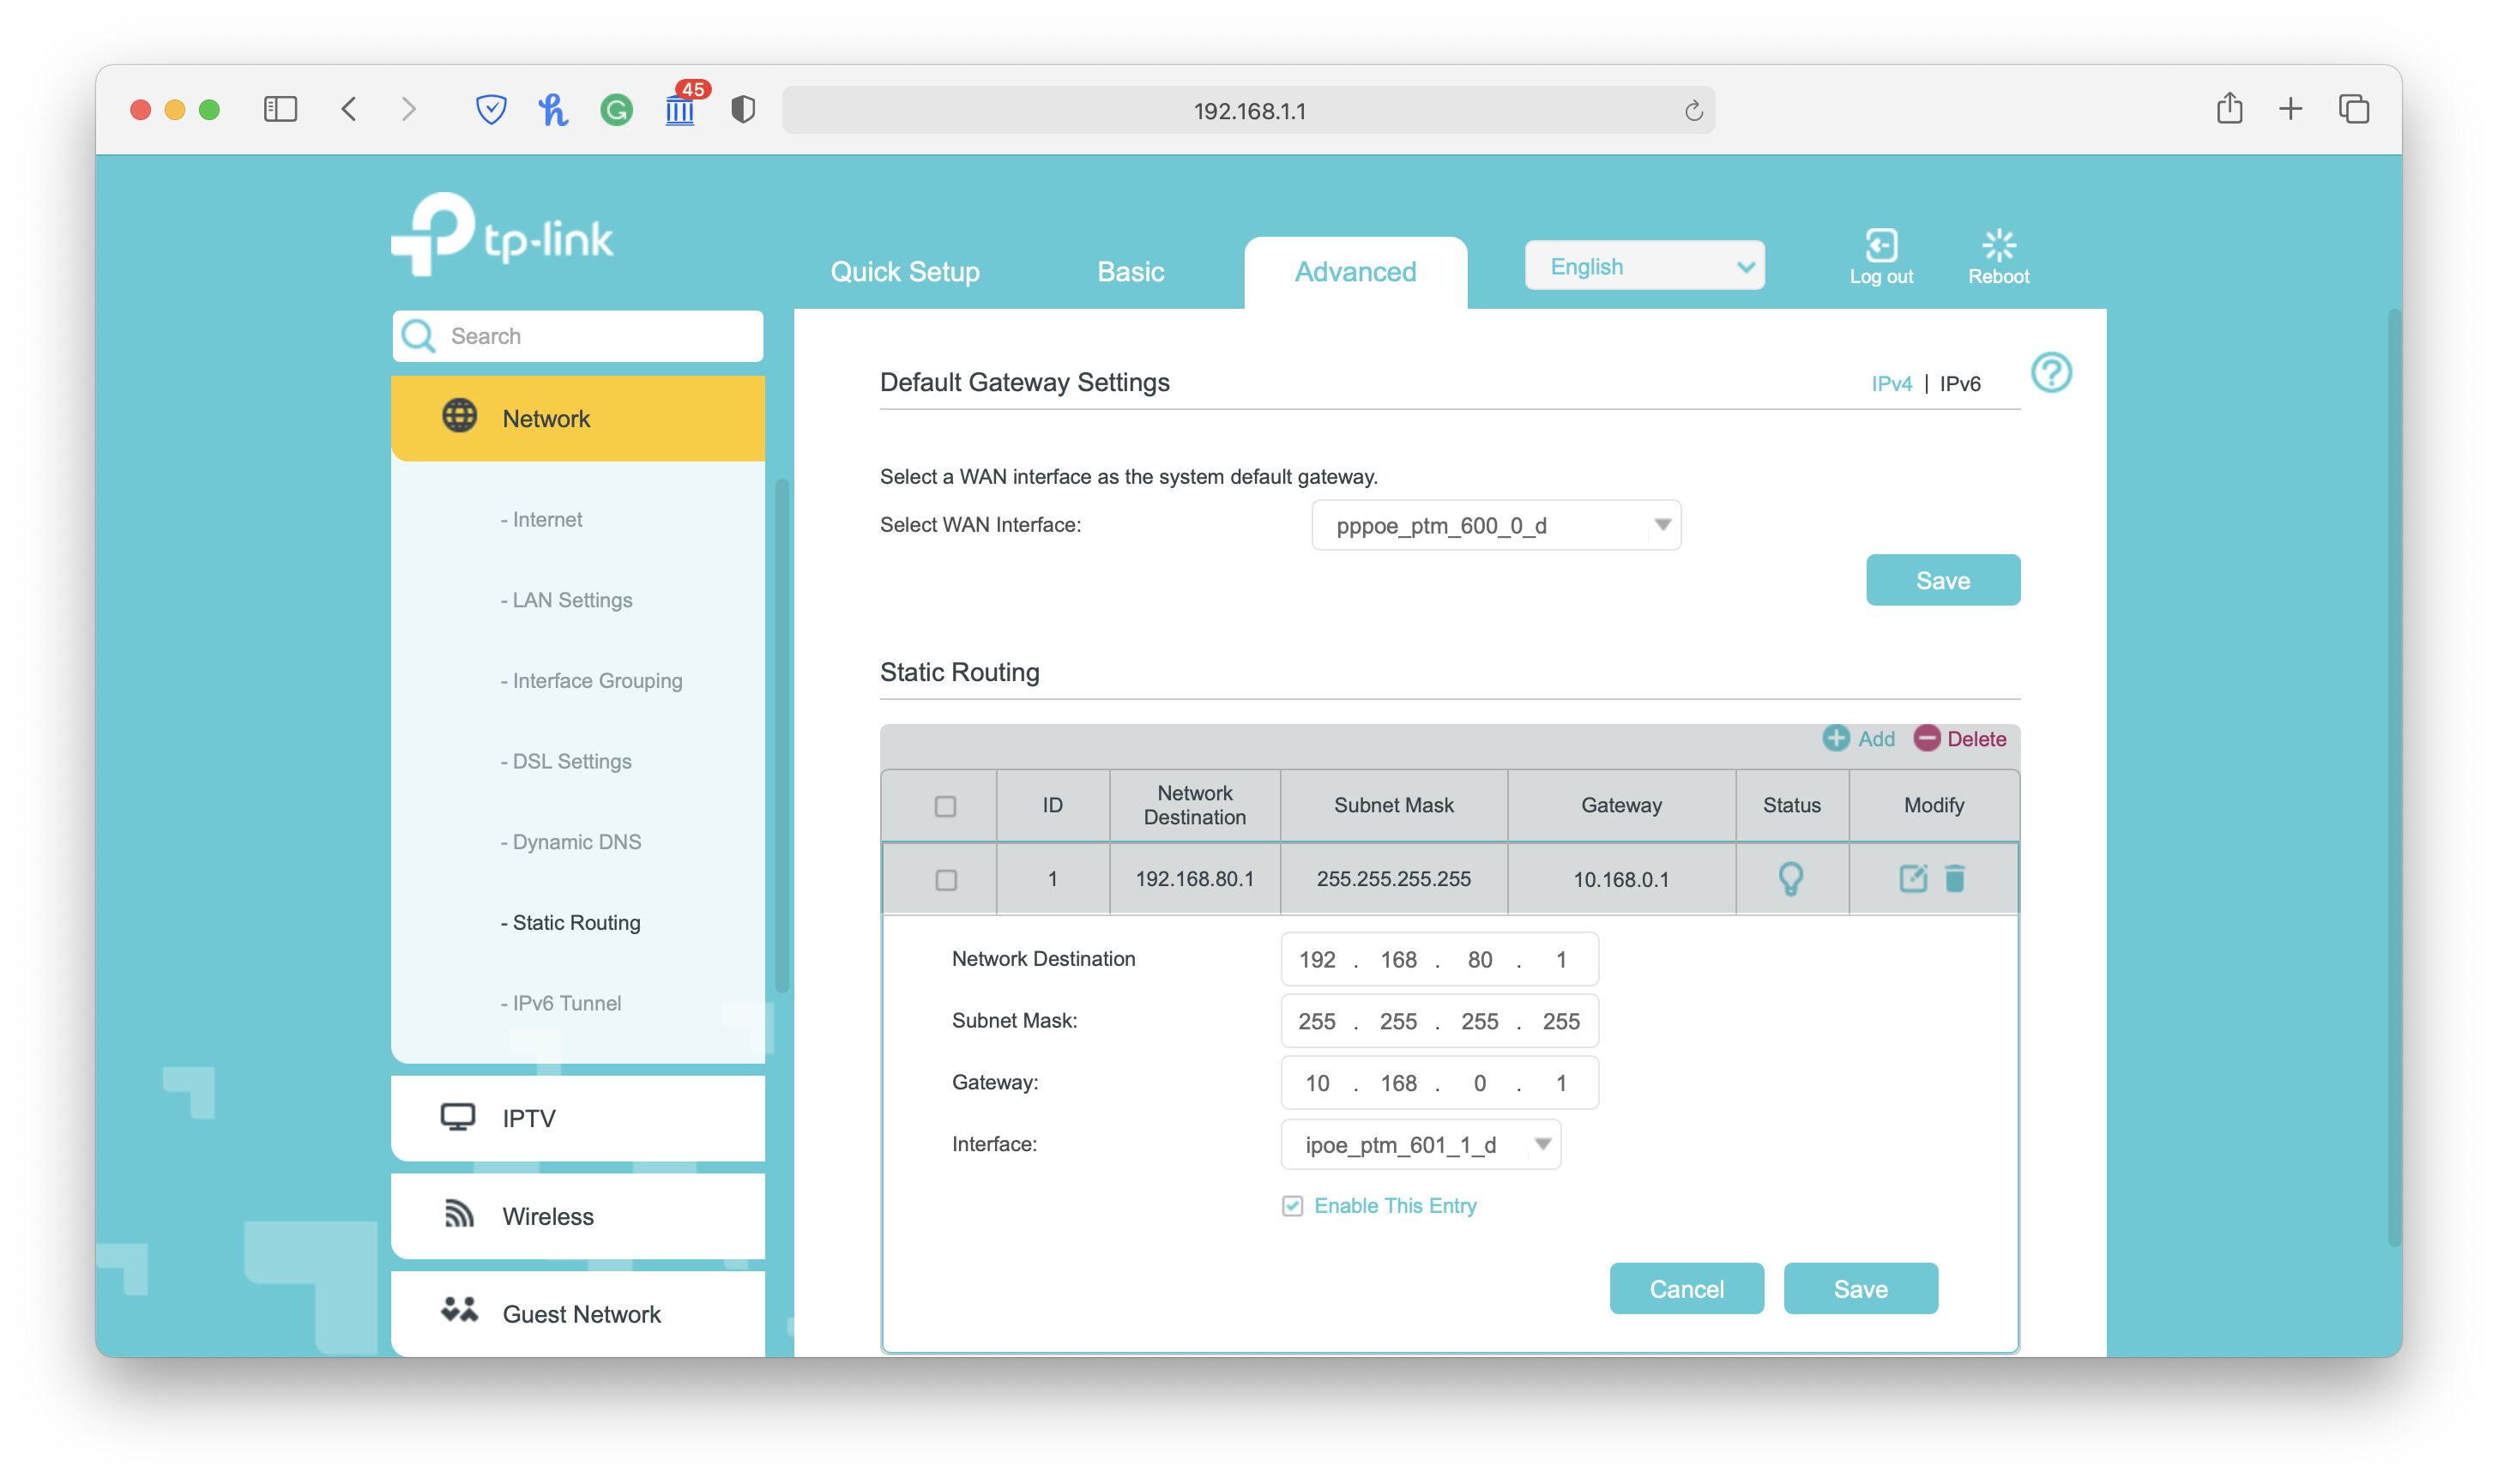
\includegraphics[width=\linewidth]{contents/substituting-the-isp-cpe/voip/advanced-network-staticrouting.png}
    \caption{Static Routing Settings of the \gls{crg}s}
    \label{figure:crgs_staticrouting}
\end{figure}

As the default gateway is set to the Internet Connection previously configured, a static route must be configured to make connections to the \gls{sip} Proxy be routed to the new network. This can also be done on the advanced section of the management interface. The Network Destination and Subnet Mask must be respectively set to \url{192.168.80.1} and \url{255.255.255.255}. The gateway field must be filled with the \gls{ip} address of the gateway assigned to the device on the network with \gls{vlan} \gls{id} 601, and the interface must point to the same network as well, as shown in Figure \ref{figure:crgs_staticrouting}. The experiments show that even after 6 months and reboots, the gateway assigned never changes, allowing the static route not be reconfigured when a new connection is established.

\begin{figure}[h]
    \centering
    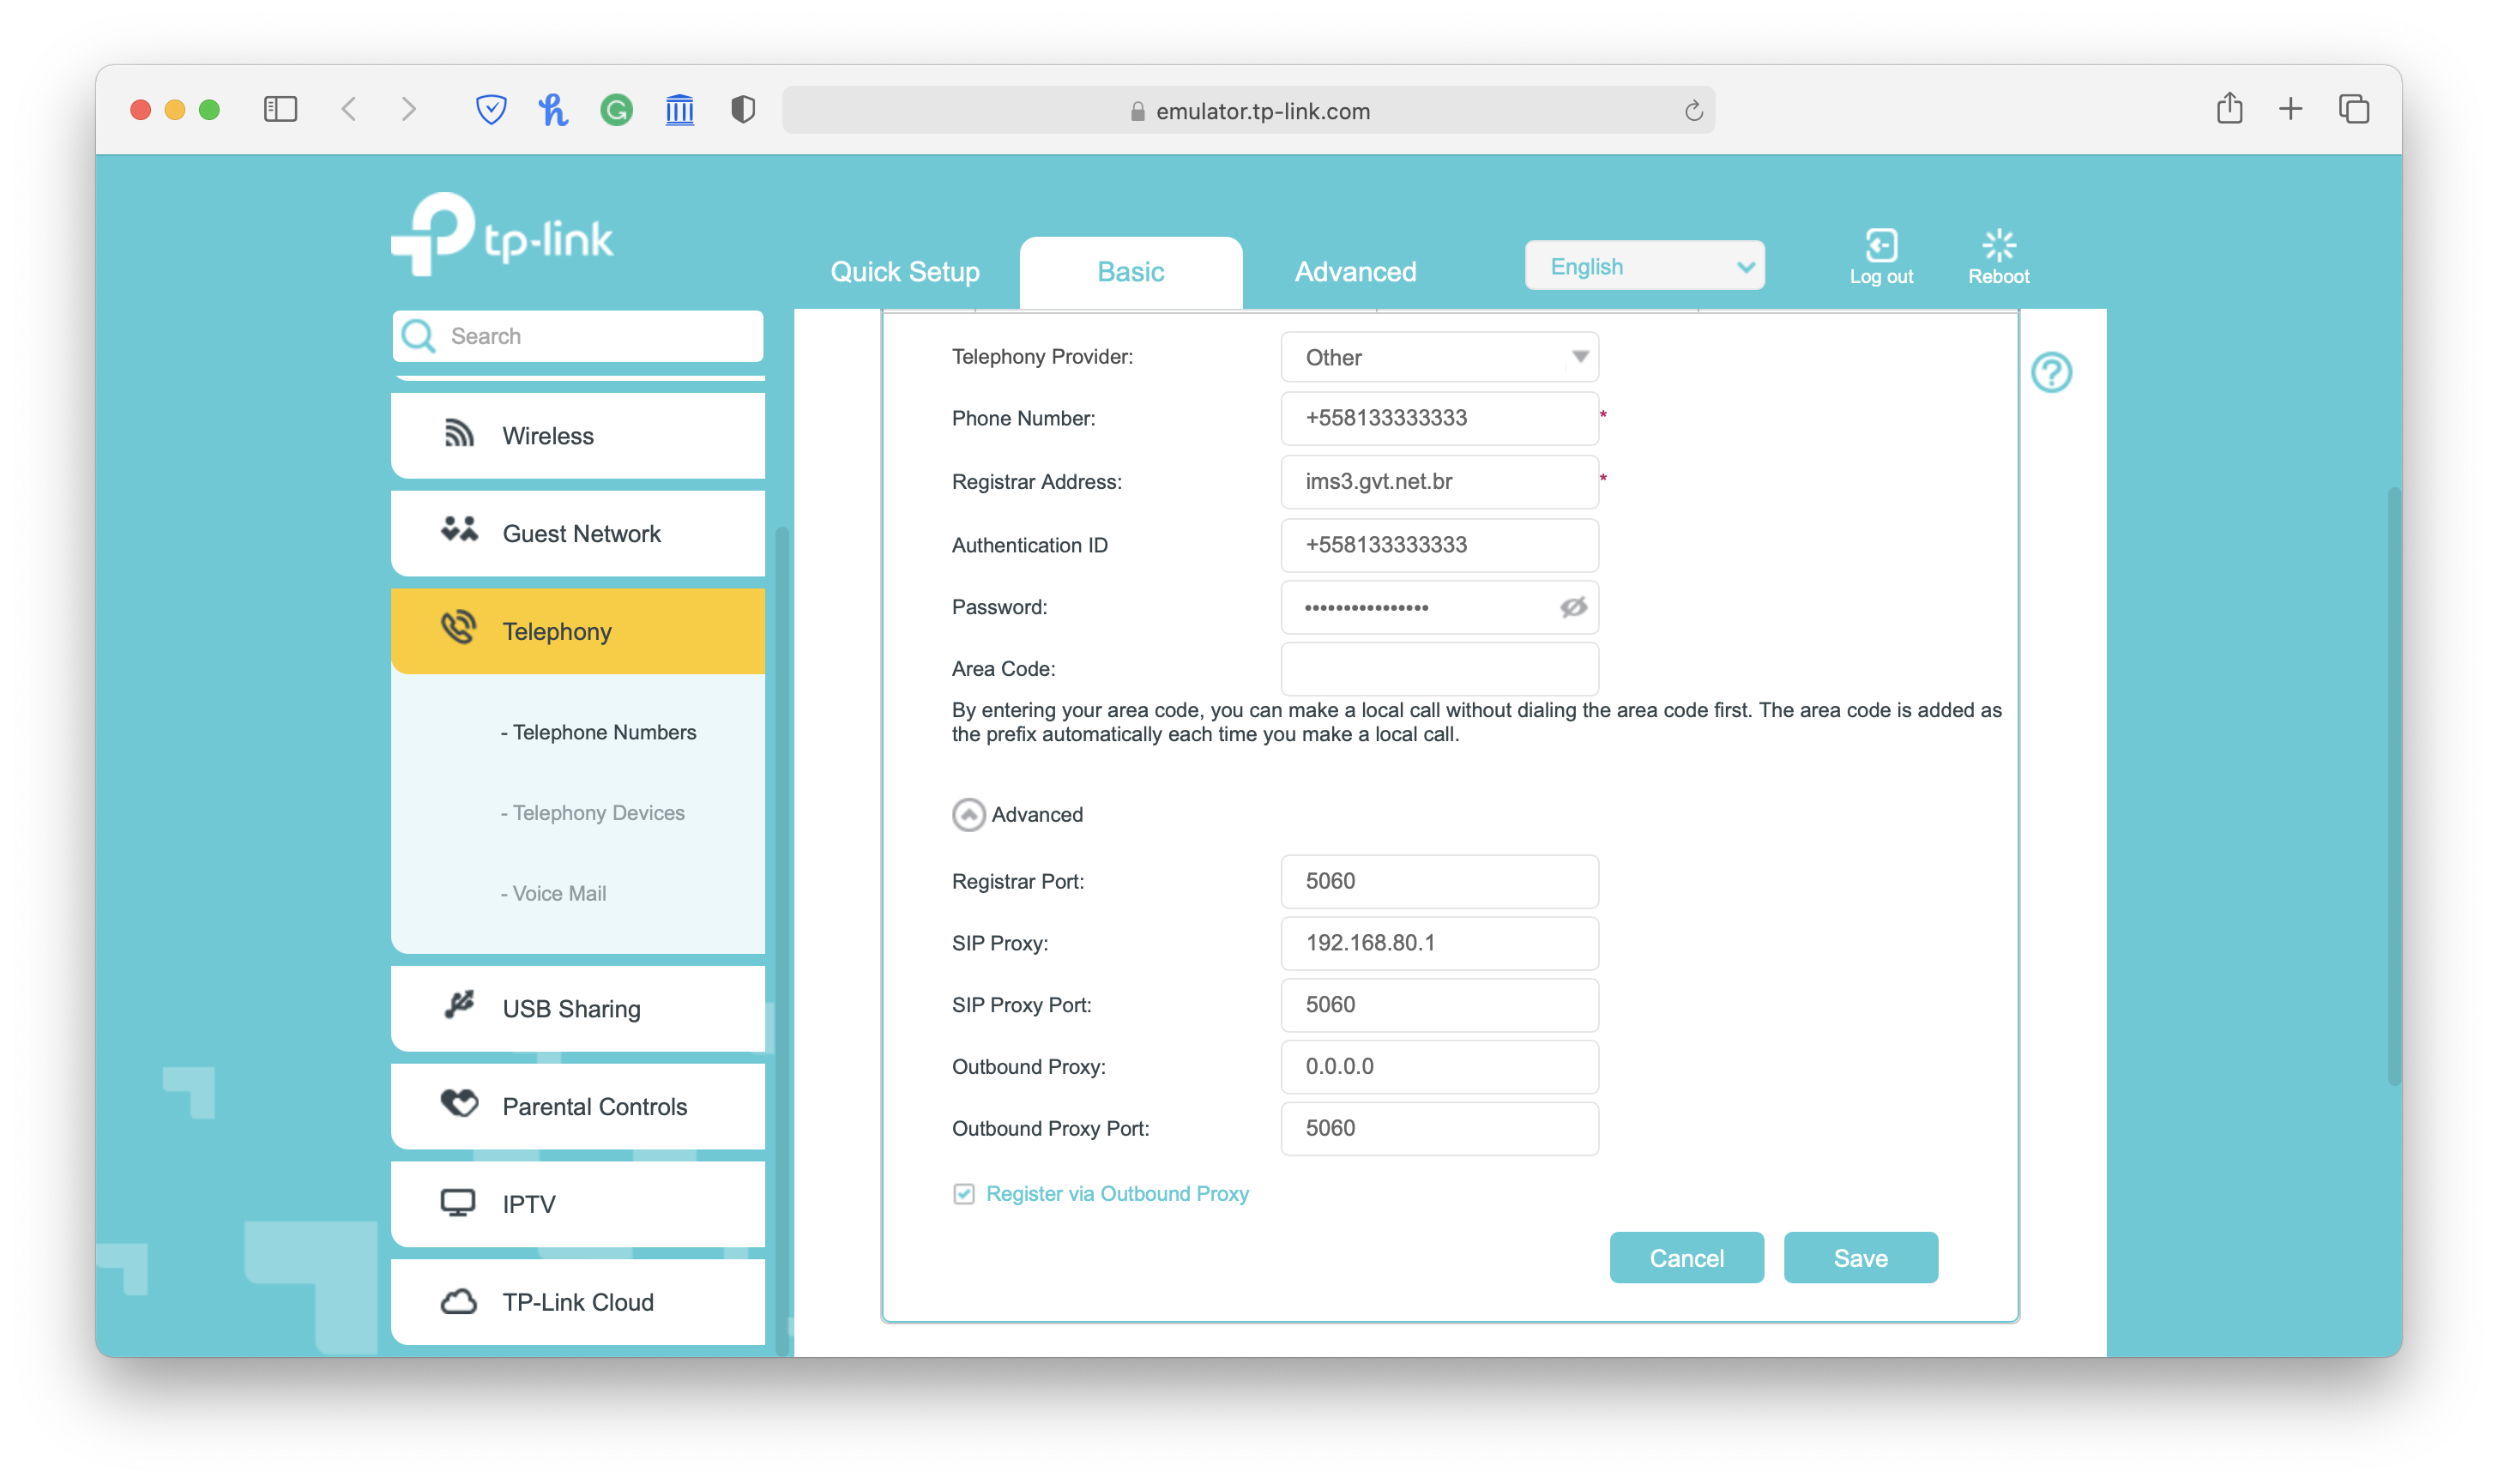
\includegraphics[width=\linewidth]{contents/substituting-the-isp-cpe/voip/basic-telephony-telephonenumbers.png}
    \caption{Telephone Numbers Settings of the \gls{crg}s}
    \label{figure:crgs_telephonenumbers}
\end{figure}

With the \gls{voip} Connection configured, a \gls{sip} client can be configured on the \gls{crg} itself, allowing analog telephones to work when connected to the \gls{rj11} ports. On the basic section of the \gls{http} Management Interface, telephone numbers can be registered. The Phone Number and Authentication \gls{id} must be set to the customer’s phone number formatted following the E.164 standard. The Registrar Address and Password are set to the values acquired from the \gls{isp} \gls{cpe} originally used by the customer. Finally, the Outbound Proxy is set to \url{192.168.80.1}, keeping the Outbound Proxy Port value of 5060 and the Register via Outbound Proxy checkbox enabled. The settings are shown in Figure \ref{figure:crgs_telephonenumbers}.

After the phone number was properly registered, the connection status showed a blue check. An analog phone was connected to the \gls{rj11} port and a number was dialed. Unfortunately the connection was unreliable, sometimes the call was successful, but most of the time there was a problem. The dialer could listen but could not be heard, the opposite also happened. After hanging a call, the number could not receive or make calls for some minutes. The phone rang indefinitely, even when out of the hook.

To diagnose the problem, a \gls{sip} client was used on a computer instead of using the \gls{crg} one. This should work fine, because differently from the \gls{isp} \gls{cpe}s, the \gls{crg} is not configured to block connections going to the \gls{sip} proxy. The Telephone app was used as \gls{sip} client, as it was free and open source. But after setting the connection on it, similar problems arose.

As it was unlikely that both \gls{sip} clients were not properly implemented, the \gls{sip} traffic of the \gls{crg} the the client running on the computer were captured and compared with the traffic previously captured from the \gls{sip} \gls{cpe}. Everything looked very similar but with one subtle difference, the \gls{sip} clients from the \gls{crg} and the computer were sending keep-alive requests to the \gls{sip} server, while the \gls{cpe} wasn’t sending them.

Looking at the implementation of the computer and \gls{crg} clients, it was found that they use the PJSIP to establish and manage the \gls{sip} connection. The \gls{crg} used the PJSIP \gls{cli}, while the computer client used the PJSIP library. Both are configured by default to send \gls{cr}-\gls{lf} as keep-alive packets every 15 seconds.

The Telephone app is recompiled with a configuration that prevents those keep-alive requests from being sent. After doing that, the \gls{sip} client started to work perfectly, just like the \gls{sip} \gls{cpe}, confirming the problem was indeed the keep-alive packets.

Unfortunately the \glspl{crg} have no configuration that allows keep-alive to be disabled. Additionally, the PJSUA \gls{cli} doesn’t have this flag either, so the PJSUA library should be used instead to allow this configuration to be changed. The firmware of the devices are closed-source, so it is not easy to build a new firmware with the changes required.

While looking for alternatives, it was found that both \glspl{crg} have iptables installed on them and have the necessary modules installed to filter the keep-alive packages going to the \gls{sip} proxy. The devices were restarted without the copper or fiber cables connected to them, preventing any connection from being established. Then the \gls{ssh} Management Interface was accessed and iptables rule was created, dropping the \gls{sip} keep-alive packets. The copper and fiber cables were reconnected and the connection established. From that point, although the \gls{sip} client was still sending the problematic packets, the \gls{sip} server never received them and the service started working just like the modified Telephone app.

\begin{lstlisting}[language=Bash,numbers=left]
iptables -I OUTPUT -p udp -j DROP -d 192.168.80.1 -m udp --dport 5060 -m string --hex-string '|0d0a|' --algo bm --from 28 --to 30
\end{lstlisting}

The solution found is untethered and the processed needs to be executed every time the \gls{crg} reboots. But it is feasible to use if the device is not rebooted frequently, or if a computer that is always connected to it via a wired connection is able to automatically execute the process every time the connection is lost and then reestablished. Another possibility would be having the \gls{sip} proxy point to a device that drops the keep-alive packets and then forward to the real \gls{sip} proxy.

It is important to notice that the \gls{crg} doesn’t need to support \gls{voip} if a \gls{sip} client running on another device can be used in the desired scenario, it just needs to be able to establish a connection with the proper \gls{vlan} \gls{id} and Connection Type. This also means that consumers can acquire cheaper \glspl{crg} that don’t have \gls{voip} built-in and use other solutions that fit in the use-case, like an external \gls{ata}.

\FloatBarrier
